\documentclass[a4paper,12pt,twocolumn]{report}
\usepackage[utf8]{inputenc}
\usepackage{graphicx}
\usepackage{natbib}   % omit 'round' option if you prefer square brackets
\usepackage{hyperref}
\graphicspath{ {imgs/} }


%opening
\title{Effects of Swarming on Learning Rate of a Population}
\author{Dominic Hauton}



\begin{document}
\maketitle
\bibliographystyle{plainnat}

\section{Introduction}
In this research we will attempt to reproduce the findings of \cite{powell2009late}'s findings using a modified version of \cite{henrich2004demography}'s transmission model. We are looking to find the benefits of a more social population, which we simulate through swarming behaviour.

If \cite{powell2009late}'s findings are correct, we should observe faster knowledge increase, higher proportion of movement individuals opt to socialise. As individuals develop and share better ways to consume resources, they will be able to live in higher densities, leading to an exponential increase in learning.

\section{Signalling}
In following \cite{henrich2004demography}'s model, turtles learn incorrectly more often than they learn correctly, leading to a general drop in knowledge, but will choose to learn from the individual with the highest level of knowledge in range.

The first semantic modification, is the turtles learn by observation which is done to simulate observing how an individual would forage in the vicinity. To prevent instant propagation of knowledge through a population, at best a turtle would only half the knowledge difference from teacher.

\section{Methodology}
To simulate a swarming behaviour, turtles will forage for food until they gain a certain level of energy, at this point they will meander to the highest concentration of turtles within visible distance. Note; this distance is higher than the observation distance, so turtles benefit from wandering into a more populus area, at the risk of finding less food. This is a simplified version of the three-zones model used by \cite{1982simulation} and \cite{huth1992simulation}, where velocity of the group is ignored, to prevent swarms colliding and coalescing.

We will vary the probability of a turtle meandering towards a more populated area during experimentation, thereby simulating the willingness of an individual to socialise. In fig \ref{fig:swarming} the effect of changing this probabilty can be observed.

\begin{figure}[b]
 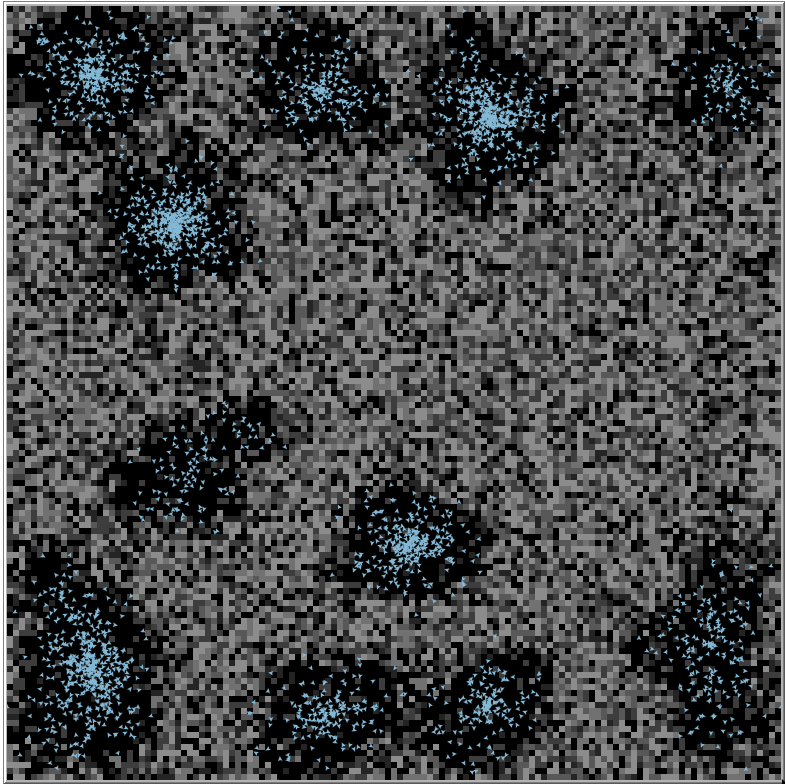
\includegraphics[width=0.24\textwidth]{swarming-high}
 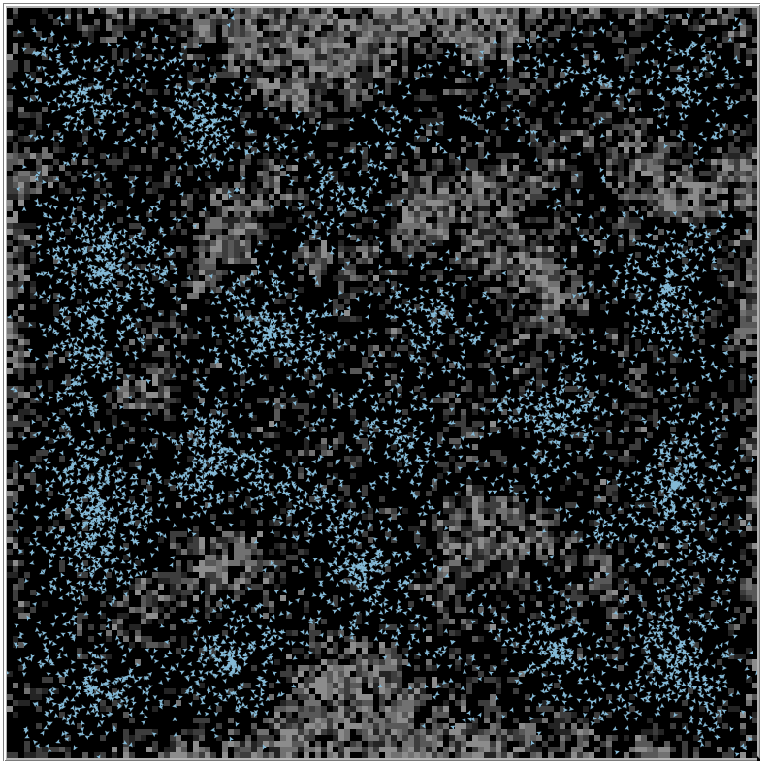
\includegraphics[width=0.24\textwidth]{swarming-low}
 \caption{Swarming Levels - 1.0 \& 0.8 resp.}
 \label{fig:swarming}
\end{figure}

The simulation is performed in Netlogo 6.0 and the relevant code has been provided, forked from a similar project by \cite{vcavce2007agent}. 50 runs of simulation will be performed for each tested swarming probability.

\section{Results}

The results of the simulation show an expected and statistically significant increase (using a p-value of 0.05) in knowledge progression within the population. Fig \ref{fig:table} shows the ideal knowledge progression occuring when turtles spent all of the time they were full in the swarm, only venturing out when hungry. There was no knowledge progression with a swarming rate of 0.7 and values below dipped initially, but quickly became insignifiant, so we use 0.7 as our base reading.

\begin{figure}
 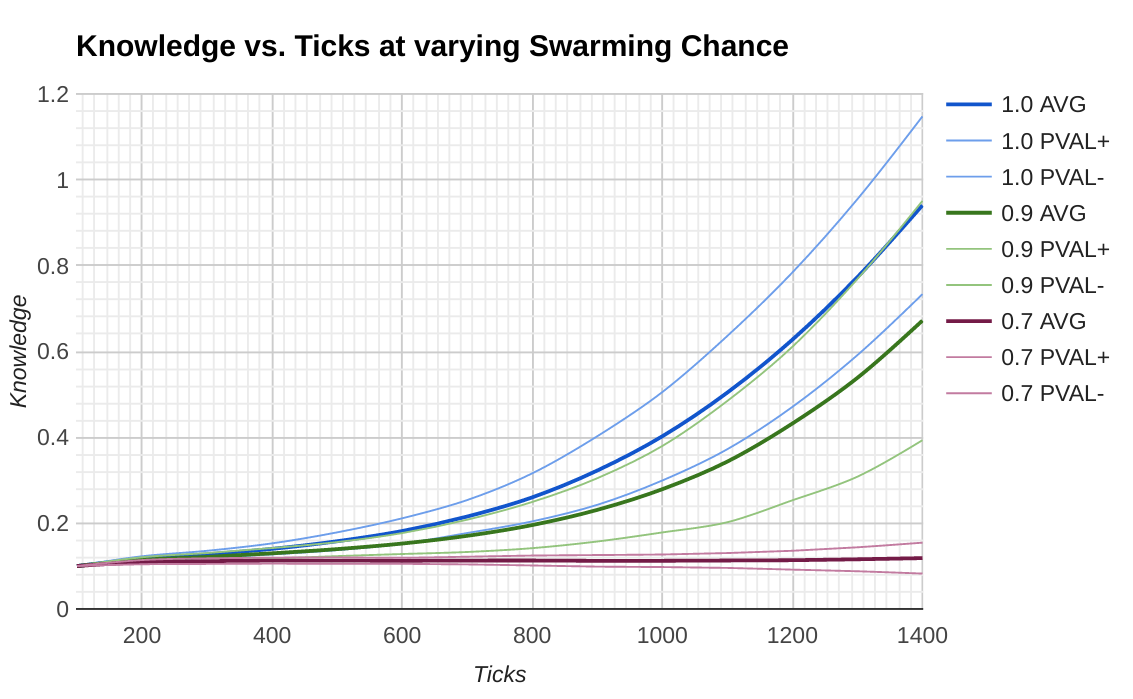
\includegraphics[width=0.5\textwidth]{swarming-effect}
 \caption{Knowledge vs Time - Results}
 \label{fig:table}
\end{figure}

An interesting observation was that fertile ground was required for swarming without the repulsion factor described by \cite{agueh2011analysis}.

When the food replacement rate was dropped past a critical point the swarming behaviour led to sudden death within the swarm as the members couldn't get out of the highly populated area fast enough to eat. When the swarm died the knowledge with it was lost.

\section{Conclusion}

This sudden death might well be cause of sparks of intelligence observed during the Upper Paleolithic transion, as described by \cite{powell2009late}. 

\bibliography{biblio1}

\end{document}
